%%%%%%%%%%%%%%%%%%%%%%%%%%%%%%%%%%%%%%%%%
% Masters/Doctoral Thesis 
% LaTeX Template
% Version 2.5 (27/8/17)
%
% This template was downloaded from:
% http://www.LaTeXTemplates.com
%
% Version 2.x major modifications by:
% Vel (vel@latextemplates.com)
%
% This template is based on a template by:
% Steve Gunn (http://users.ecs.soton.ac.uk/srg/softwaretools/document/templates/)
% Sunil Patel (http://www.sunilpatel.co.uk/thesis-template/)
%
% Template license:
% CC BY-NC-SA 3.0 (http://creativecommons.org/licenses/by-nc-sa/3.0/)
%
%%%%%%%%%%%%%%%%%%%%%%%%%%%%%%%%%%%%%%%%%

%----------------------------------------------------------------------------------------
%	PACKAGES AND OTHER DOCUMENT CONFIGURATIONS
%----------------------------------------------------------------------------------------

\documentclass[
11pt, % The default document font size, options: 10pt, 11pt, 12pt
%oneside, % Two side (alternating margins) for binding by default, uncomment to switch to one side
english, % ngerman for German
singlespacing, % Single line spacing, alternatives: onehalfspacing or doublespacing
%draft, % Uncomment to enable draft mode (no pictures, no links, overfull hboxes indicated)
%nolistspacing, % If the document is onehalfspacing or doublespacing, uncomment this to set spacing in lists to single
%liststotoc, % Uncomment to add the list of figures/tables/etc to the table of contents
%toctotoc, % Uncomment to add the main table of contents to the table of contents
%parskip, % Uncomment to add space between paragraphs
%nohyperref, % Uncomment to not load the hyperref package
headsepline, % Uncomment to get a line under the header
%chapterinoneline, % Uncomment to place the chapter title next to the number on one line
%consistentlayout, % Uncomment to change the layout of the declaration, abstract and acknowledgements pages to match the default layout
]{MastersDoctoralThesis} % The class file specifying the document structure

\usepackage[utf8]{inputenc} % Required for inputting international characters
\usepackage[T1]{fontenc} % Output font encoding for international characters

\usepackage{mathpazo} % Use the Palatino font by default

\usepackage[backend=bibtex,style=authoryear,natbib=true]{biblatex} % Use the bibtex backend with the authoryear citation style (which resembles APA)

\addbibresource{example.bib} % The filename of the bibliography

\usepackage[autostyle=true]{csquotes} % Required to generate language-dependent quotes in the bibliography

%----------------------------------------------------------------------------------------
%	MARGIN SETTINGS
%----------------------------------------------------------------------------------------

\geometry{
	paper=a4paper, % Change to letterpaper for US letter
	inner=2.5cm, % Inner margin
	outer=3.8cm, % Outer margin
	bindingoffset=.5cm, % Binding offset
	top=1.5cm, % Top margin
	bottom=1.5cm, % Bottom margin
	%showframe, % Uncomment to show how the type block is set on the page
}

%----------------------------------------------------------------------------------------
%	THESIS INFORMATION
%----------------------------------------------------------------------------------------

\thesistitle{Implementation of a robot behavior learning simulator} % Your thesis title, this is used in the title and abstract, print it elsewhere with \ttitle
\supervisor{Dr. Mihaela \textsc{JUGANARU-MATHIEU}} % Your supervisor's name, this is used in the title page, print it elsewhere with \supname
\examiner{} % Your examiner's name, this is not currently used anywhere in the template, print it elsewhere with \examname
\degree{Master's 1 in Cyber-Physical and Social Systems} % Your degree name, this is used in the title page and abstract, print it elsewhere with \degreename
\author{Kushagra Singh \textsc{BISEN}} % Your name, this is used in the title page and abstract, print it elsewhere with \authorname
\addresses{} % Your address, this is not currently used anywhere in the template, print it elsewhere with \addressname

\subject{Biological Sciences} % Your subject area, this is not currently used anywhere in the template, print it elsewhere with \subjectname
\keywords{} % Keywords for your thesis, this is not currently used anywhere in the template, print it elsewhere with \keywordnames
\university{\href{https://www.mines-stetienne.fr/}{école nationale supérieure des mines de saint-étienne}} % Your university's name and URL, this is used in the title page and abstract, print it elsewhere with \univname
\department{\href{https://www.mines-stetienne.fr/recherche/departements/departement-informatique-et-systemes-intelligents/}{Institu Henri Fayol, IT and Intelligent Systems department}} % Your department's name and URL, this is used in the title page and abstract, print it elsewhere with \deptname
\group{\href{http://researchgroup.university.com}{Set of Intelligent Robots Project}} % Your research group's name and URL, this is used in the title page, print it elsewhere with \groupname
\faculty{\href{http://faculty.university.com}{Faculty Name}} % Your faculty's name and URL, this is used in the title page and abstract, print it elsewhere with \facname

\AtBeginDocument{
\hypersetup{pdftitle=\ttitle} % Set the PDF's title to your title
\hypersetup{pdfauthor=\authorname} % Set the PDF's author to your name
\hypersetup{pdfkeywords=\keywordnames} % Set the PDF's keywords to your keywords
}

\begin{document}

\frontmatter % Use roman page numbering style (i, ii, iii, iv...) for the pre-content pages

\pagestyle{plain} % Default to the plain heading style until the thesis style is called for the body content

%----------------------------------------------------------------------------------------
%	TITLE PAGE
%----------------------------------------------------------------------------------------

\begin{titlepage}
\begin{center}

\vspace*{.06\textheight}
{\scshape\LARGE \univname\par}\vspace{1.5cm} % University name
\textsc{\Large Master's 1 Report}\\[0.5cm] % Thesis type

\HRule \\[0.4cm] % Horizontal line
{\huge \bfseries \ttitle\par}\vspace{0.4cm} % Thesis title
\HRule \\[1.5cm] % Horizontal line
 
\begin{minipage}[t]{0.4\textwidth}
\begin{flushleft} \large
\emph{Author:}\\
\href{https://argahsuknesib.github.io/}{\authorname} % Author name - remove the \href bracket to remove the link
\end{flushleft}
\end{minipage}
\begin{minipage}[t]{0.4\textwidth}
\begin{flushright} \large
\emph{Supervisor:} \\
\href{http://www.jamessmith.com}{\supname} % Supervisor name - remove the \href bracket to remove the link  
\end{flushright}
\end{minipage}\\[3cm]
 
\vfill

\large \textit{A thesis submitted in fulfillment of the requirements\\ for the degree of \degreename}\\[0.3cm] % University requirement text
\textit{in the}\\[0.4cm]
\groupname\\\deptname\\[2cm] % Research group name and department name
 
\vfill

{\large \today}\\[4cm] % Date
%\includegraphics{Logo} % University/department logo - uncomment to place it
 
\vfill
\end{center}
\end{titlepage}

%----------------------------------------------------------------------------------------
%	DECLARATION PAGE
%----------------------------------------------------------------------------------------

\begin{declaration}
\addchaptertocentry{\authorshipname} % Add the declaration to the table of contents
\noindent I, \authorname, declare that this thesis titled, \enquote{\ttitle} and the work presented in it are my own. I confirm that:

\begin{itemize} 
\item This work was done wholly or mainly while in candidature for a research degree at this University.
\item Where any part of this thesis has previously been submitted for a degree or any other qualification at this University or any other institution, this has been clearly stated.
\item Where I have consulted the published work of others, this is always clearly attributed.
\item Where I have quoted from the work of others, the source is always given. With the exception of such quotations, this thesis is entirely my own work.
\item I have acknowledged all main sources of help.
\item Where the thesis is based on work done by myself jointly with others, I have made clear exactly what was done by others and what I have contributed myself.\\
\end{itemize}
 
\noindent Signed:\\
\rule[0.5em]{25em}{0.5pt} % This prints a line for the signature
 
\noindent Date:\\
\rule[0.5em]{25em}{0.5pt} % This prints a line to write the date
\end{declaration}

\cleardoublepage

%----------------------------------------------------------------------------------------
%	QUOTATION PAGE
%----------------------------------------------------------------------------------------

\vspace*{0.2\textheight}

\noindent\enquote{\itshape Thanks to my solid academic training, today I can write hundreds of words on virtually any topic without possessing a shred of information, which is how I got a good job in journalism.}\bigbreak

\hfill Dave Barry

%----------------------------------------------------------------------------------------
%	ABSTRACT PAGE
%----------------------------------------------------------------------------------------

\begin{abstract}
\addchaptertocentry{\abstractname} % Add the abstract to the table of contents
The Thesis Abstract is written here (and usually kept to just this page). The page is kept centered vertically so can expand into the blank space above the title too\ldots
\end{abstract}

%----------------------------------------------------------------------------------------
%	ACKNOWLEDGEMENTS
%----------------------------------------------------------------------------------------

\begin{acknowledgements}
\addchaptertocentry{\acknowledgementname} % Add the acknowledgements to the table of contents
The acknowledgments and the people to thank go here, don't forget to include your project advisor\ldots
\end{acknowledgements}

%----------------------------------------------------------------------------------------
%	LIST OF CONTENTS/FIGURES/TABLES PAGES
%----------------------------------------------------------------------------------------

\tableofcontents % Prints the main table of contents

\listoffigures % Prints the list of figures

\listoftables % Prints the list of tables

%----------------------------------------------------------------------------------------
%	ABBREVIATIONS
%----------------------------------------------------------------------------------------

\begin{abbreviations}{ll} % Include a list of abbreviations (a table of two columns)

\textbf{LAH} & \textbf{L}ist \textbf{A}bbreviations \textbf{H}ere\\
\textbf{WSF} & \textbf{W}hat (it) \textbf{S}tands \textbf{F}or\\

\end{abbreviations}

%----------------------------------------------------------------------------------------
%	PHYSICAL CONSTANTS/OTHER DEFINITIONS
%----------------------------------------------------------------------------------------

\begin{constants}{lr@{${}={}$}l} % The list of physical constants is a three column table

% The \SI{}{} command is provided by the siunitx package, see its documentation for instructions on how to use it

Speed of Light & $c_{0}$ & \SI{2.99792458e8}{\meter\per\second} (exact)\\
%Constant Name & $Symbol$ & $Constant Value$ with units\\

\end{constants}

%----------------------------------------------------------------------------------------
%	SYMBOLS
%----------------------------------------------------------------------------------------

\begin{symbols}{lll} % Include a list of Symbols (a three column table)

$a$ & distance & \si{\meter} \\
$P$ & power & \si{\watt} (\si{\joule\per\second}) \\
%Symbol & Name & Unit \\

\addlinespace % Gap to separate the Roman symbols from the Greek

$\omega$ & angular frequency & \si{\radian} \\

\end{symbols}

%----------------------------------------------------------------------------------------
%	DEDICATION
%----------------------------------------------------------------------------------------

\dedicatory{For/Dedicated to/To my\ldots} 

%----------------------------------------------------------------------------------------
%	THESIS CONTENT - CHAPTERS
%----------------------------------------------------------------------------------------

\mainmatter % Begin numeric (1,2,3...) page numbering

\pagestyle{thesis} % Return the page headers back to the "thesis" style

% Include the chapters of the thesis as separate files from the Chapters folder
% Uncomment the lines as you write the chapters


% Chapter Template

\chapter{Context} % Main chapter title

\label{ChapterX} % Change X to a consecutive number; for referencing this chapter elsewhere, use \ref{ChapterX}

%----------------------------------------------------------------------------------------
%	SECTION 1
%----------------------------------------------------------------------------------------

\section{Introduction}
The work is based on an Industry 4.0 scenario, which is a cyber-physical environment consisting of various different 
actors and objects involved. The different actors involved are either stationary or mobile. Moreover, complexity of the 
environment increases when we account for heterogeneous actors with various decision making capabilities. Robots with various
manufacturers present various transform frames, different software and sensors. Due to the heterogeneous nature of the robots 
involved, we can not depend on information we receive from the robot, as this particular information will differ from a robot 
to other based upon it's configuration. The problem is solved by creating a digital twin which records the information of the 
environment as well as the robot. The simulator notes the state of the robot and obstacles it surrounds as it passes 
through the obstacle grid. 
\subsection{Motivation}
The structure of a dynamic Industry 4.0 environment is highly volatile, the structure is defined through a stationary frame that 
has been declared before. The decision making capabilities of the robot to navigate the environment while avoiding obstacles and 
other robots can have a great impact on the performance and the utility of the environment. 

% % Chapter Template

\chapter{Technologies Used} % Main chapter title

\label{Chapter2} % Change X to a consecutive number; for referencing this chapter elsewhere, use \ref{ChapterX}

\section{Introduction}
In the previous chapter, we went over an introduction to the context of the work as well as the methods through which we can accomplish the goal of learning the behaviour of the robot as it moves in the configuration space.
As we know a basic introduction to the work,  in this chapter we would go over the technologies that are employed to achieve the goal of learning the behaviour of the robot. We will first go over the hardware and software requirements of the robot, and the environment.
\section{Hardware Employed}
The project uses a Turtlebot2 \cite{t2} robot. Turtlebot2 (see Figure~\ref{fig:Turtlebot2}) is a low-cost, personal robot kit with open-sourced software. The robot was created in 2010, but has been continuously envolved in both 
software strength and hardware with open-source contributions to the project. The Turtlebot2 consists of a base, two wheels, a single board computer and a LIDAR sensor. Other sensors for example a vision sensor, i.e. Camera can be attached later to the mainframe based upon the requirement.
Turtlebot2 accomplishes SLAM and Navigation efficiently in the configuration space. It is developed to be employable in various scenarios, and can be controlled remotely by a computer or a joystick. 
Turtlebot2 can be attached with an arm to perform manipulator tasks.

\begin{figure}[th]
    \centering
    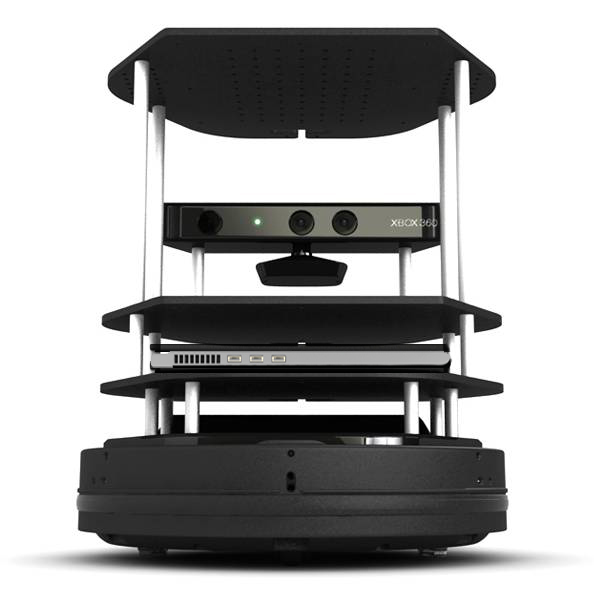
\includegraphics[width=0.5\textwidth]{Figures/turtlebot2.jpg}
    \decoRule
    \caption[]{Turtlebot2}
    \label{fig:Turtlebot2}
    \end{figure}

\subsection{LIDAR Sensor}
LIDAR stands for light detection and ranging. LIDAR sensor measures the time of flight of the pulse of light.
The light transmitted from LIDAR hits an obstacle and is noted. The light transmitted is usually infrared, where most of the energy is concentrated
in a narrow beam of light. The distance to the obstacle is calculated by measuring the time of flight in seconds.
The hardware involved here is a receiver emitter pairs (channels) which is combined wuth rotating mirrors to ensure that the whole area is covered.
They are used in autonomous devices. The sampling rate of a LIDAR is high, therefore the light beams do not collide with one another resulting in precision.
The range of LIDAR sensor are measured by maximum likelihood estimators. There are various types of LIDAR sensors with varying capabilities such as difference in the scanning area, resolution, detection range.
The resuting data collected is a point cloud grid.
\section{Software Employed}
\subsection{Gazebo Simulator}
In the implementation, we are using \textbf{Gazebo} \cite{1389727} as a simulator to visualize and execute the processes.
Gazebo is a well-designed high quality simulation software with a real physics engine. Gazebo makes it easy for researchers to test AI algorithms, design Robots, perform regression and testing and train AI systems before 
using it in real-world applications. Gazebo can use 3D models to implement real-world scenarios for the robot to interact with. It is a trusted simulator, being used by reputed space agencies to simulate robots.
Turtlebot2 has packages for Gazebo to present the robot in simulation. Gazebo's biggest advantage is it's huge community support around it.

Gazebo provides many features:
\begin{itemize}
    \item \textit{Dynamic Simulation : } Simulation is provided by many high-quality physics engine such as ODE, Bullet and DART.
    \item \textit{Advanced 3D Graphics : } Gazebo provides great simulation which is very realistic including textures, lighting and shadows.
    \item \textit{Sensors and Noise :} Simulator can be used to make real sensor data with noise from sensors and other equipments such as laser range finders, vision sensors and contact sensors etc.
    \item \textit{Plugins :} Researcher can develop custom plugin for a specific sensor or a specific task in the simulation.
    \item \textit{Robot Models: } There are many different robots which can be used in Gazebo, from simple robots such as Turtlebot2/3 to Mars Rover can be simulated in a Gazebo environment.
    \item \textit{TCP/IP Transport: } We can run simulation on remote servers, and interface with Gazebo simulator through socket based message pushing.
    \item \textit{Cloud Simulation :} CloudSim can be used to run Gazebo on Amazon Web services, or personal web service or personal architecture.
    \item \textit{Command Line Tools : } Command line tools simplify simulation control and introspection.
\end{itemize}
Gazabo11 was the version being implemented with ROS Noetic in this report's context.

\subsubsection{Environment's Entities}
In Gazebo's simulation, we get presented with a blank environment to build upon. We use Computer Aided Design (CAD) to create required entities and obstacles. In our implementation,
we had to develop boxes, tiles and borders to the environmment. The model is saved in \textit{sde} format, and rendered in Gazebo. Each box is placed at a specific position, and the borders are placed
to enclose the environment. The whole entity is made over a sheet of tile. The Gazebo environment with a turtlebot is demonstrated in the Figure~\ref{fig:GazeboTurtlebot2} 
\begin{figure}[th]
    \centering
    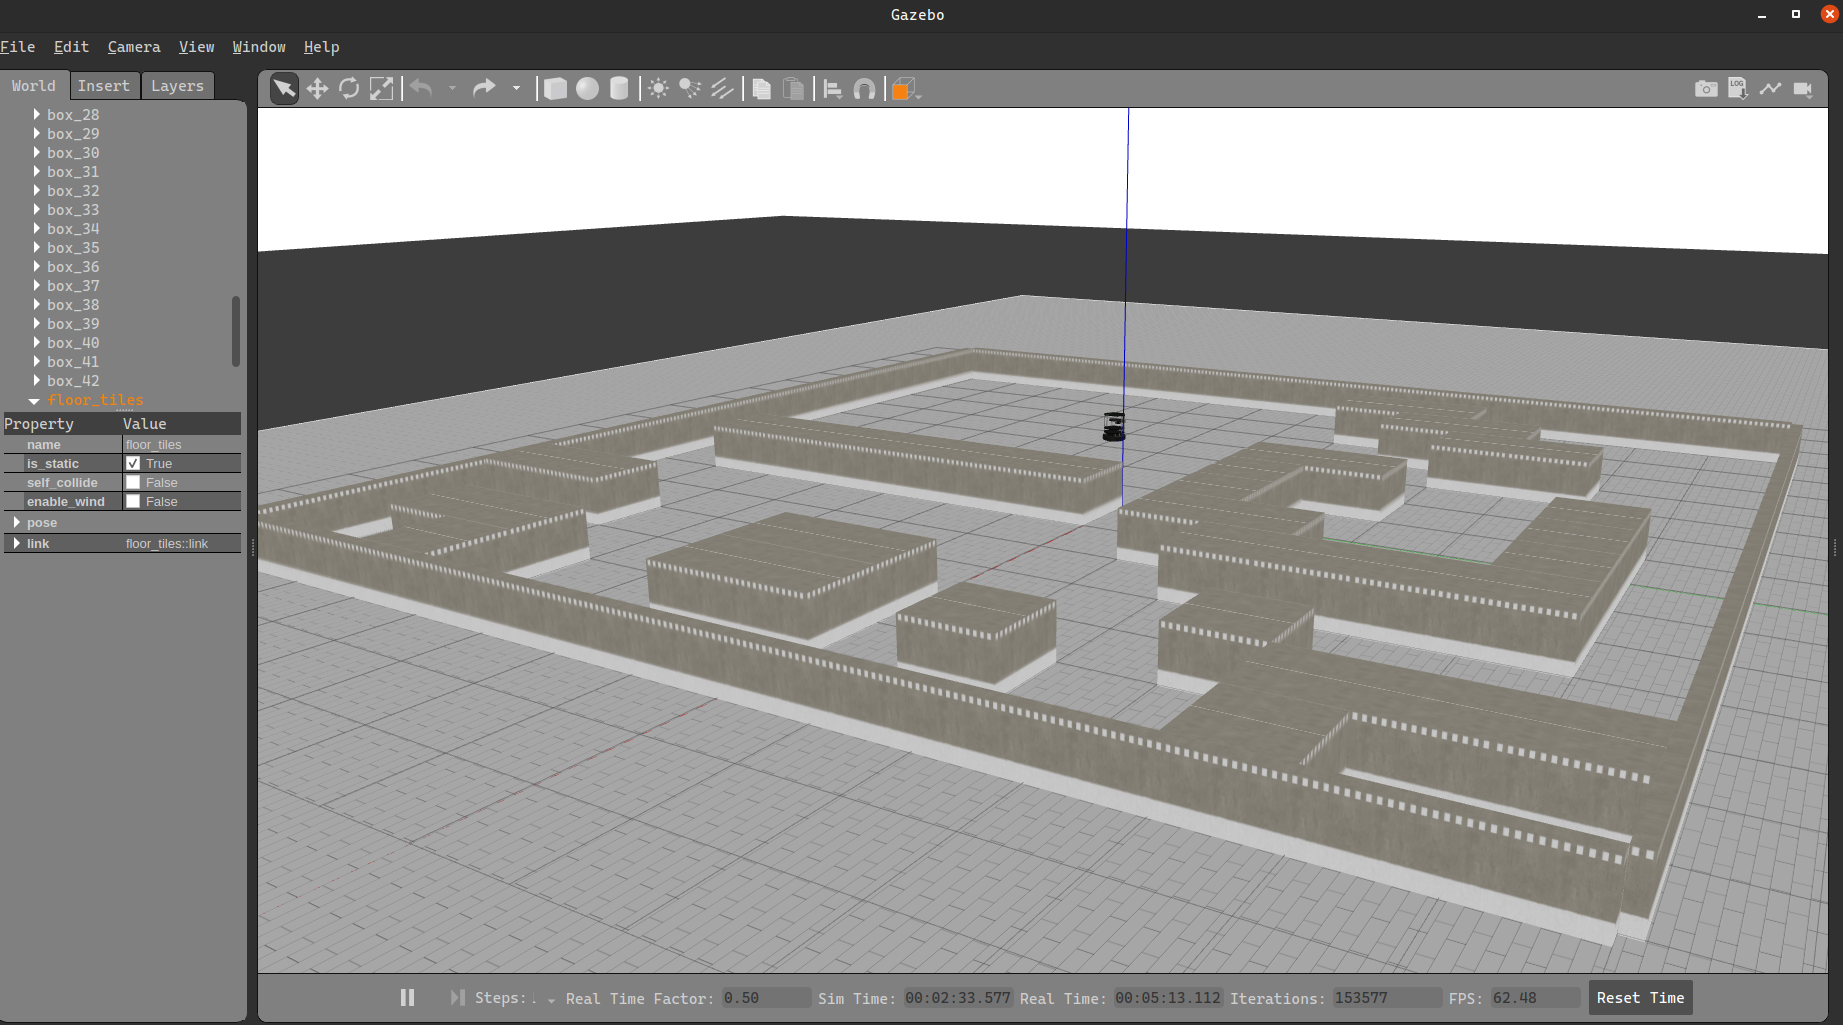
\includegraphics[width=\textwidth]{Figures/gazebo-image.png}
    \decoRule
    \caption[]{Turtlebot2 in Gazebo Environment}
    \label{fig:GazeboTurtlebot2}
\end{figure}

\section{Robot Operating System}
Robot Operating System or ROS, is known for it's flexibility as a framework to write and simulate robot software. ROS has a collection of open-source tools and libraries are used to run robots. It is
very helpful in the field of robotics as it reduces the hassle of writing and figuring most of the robot's driver and actuator code. It is at a higher level in abstraction, thus providing an option to use the same
code in simulation in Gazebo as well as to run the real robot. It provides hardware abstraction, libraries, device drivers, package management and more. 
There are various different versions of ROS, each combined with a specific version of Ubuntu's Long Term Service distribution. As the software we wish to build is supposed to be utilized later, a stable framework is a neccesity. Ubuntu 20.04 LTS and 
ROS Noetic were chosen as distributions for the project.

\subsection{ROS Packages}
In ROS, we have different packages for differnt softwares. A package is created by specific ROS commands. A ROS Package structure is : 
\begin{itemize}
    \item \textit{include/package name}: C++ scripts include headers which are stored in this directory.
    \item \textit{msg} : This folder contain msg types, i.e the types of messages being interchanged in processes.
    \item \textit{src} : This folder contains the source file for the package.
    \item \textit{srv} : This folder contains files which show the simplified service description languages.
    \item \textit{scripts} : This folder contains the scripts (in python) required to run the robot or do a specific task.
    \item \textit{CMakeLists.txt} : This file describes the ROS Package and helps the developer to specify runtime and execution time dependancies to build the catkin project.
    \item \textit{package.xml} : Describe the dependancies of the package.
    \item \textit{CHANGELOG.srt} : Many packages will define a changelog which can be automatically injected into binary packaging and into the wiki page for the package
\end{itemize}

\subsection{ROS Command Line Tools}
Packages are a central concept that are used to manage different software. Some command line tools help you to manage such packages : 
\begin{itemize}
    \item \textit{rospack} : finds and retrieves information about the package.
    \item \textit{catkin-create-pkg} : creates a new ROS package. 
    \item \textit{catkin-make} : build the workspace containing different ROS packages.
    \item \textit{rosdep} : to install the system dependencies of the package.
    \item \textit{rqt} : RQT has a  a plugin called "Introspection/Package Graph", which visualizes package dependencies as a graph.
\end{itemize} 

\section{Simulataneous Localization and Mapping}
As we studied in the previous chapter about localization, which is a process to inform the robot about it's position in the environment it is in. 
Simultaneous localization and mapping (SLAM)
is a technique applied in artificial intelligence mobile robot for
a self-exploration in numerous geographical environment.
SLAM becomes fundamental research area in recent days as it
promising solution in solving most of problems which related
to the self-exploratory oriented artificial intelligence mobile
robot field \cite{7482163}. SLAM is one of the most fundamental part of autonomous mobile robot navigation. It is used by the mobile robot to navigate around the environment 
and generate a map. The map generated is used to find the obstacle location and grid surrounding the robot to make an appropriate path planning scenario for the robot.
Although Localization and Mapping are different technologies, SLAM incorporates them together where localization is done concurrently with the robot creating the map.
The map is used to note than landmark position and be able to generate an efficient path trajectory. SLAM has the advantage of doing this together at the same time making it the most important 
algorithm in autonomous robot navigation. SLAM methods implement Extended Kalman filters. Figure~\ref{fig:SLAMFlowchart} demonstrates the SLAM process.
\begin{figure}[th]
    \centering
    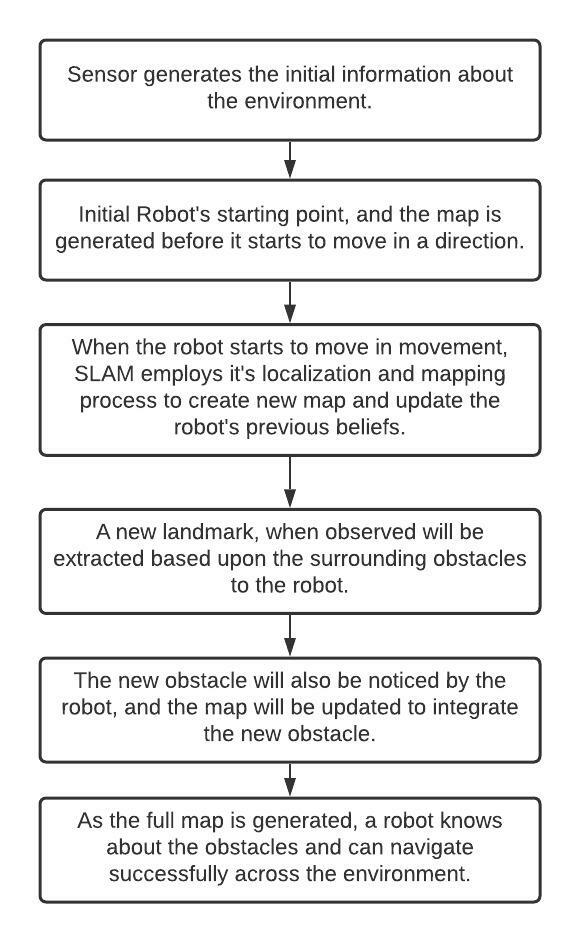
\includegraphics[width=0.5\textwidth]{Figures/SLAM_flowchart.jpeg}
    \decoRule
    \caption[]{SLAM Workflow \cite{7482163}}
    \label{fig:SLAMFlowchart}
\end{figure}
\begin{figure}[th]
    \centering
    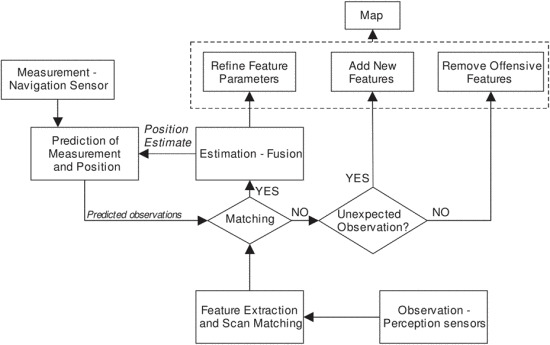
\includegraphics[width=0.8\textwidth]{Figures/SLAM_Block_Final.jpeg}
    \decoRule
    \caption[]{SLAM Block Diagram \cite{7081165}}
    \label{fig:SLAMBlockDiagram}
\end{figure}

\subsection{Features of SLAM}
Three major features of SLAM exist and are discussed below : 
\subsubsection{Mapping}
For a robot to move around autonomously in an environment. It should know where it is, providing prior knowledge. Mapping provides his capability for the robot to generate a map using the hardware sensor (mostly LIDAR) to get information from the environment.
There are various ways to represent the map, which are used to generate a path in subsequent steps. The data will be used by the robot to localize and recognize it's own position and landmark.
\subsubsection{Localization}
Localization is calculated by using the odometry of the robot. It is one of the features of SLAM which are able to calculate and estimate the poisition of the robot, and the obstacles close to it.
The mobile robot should be able to \textit{think} for itself by calculating and estimating the path travelled and calculating the nearby obstacles. 
\subsubsection{Navigation}
Navigation employs both Mapping and Localization, by combining the results of both. When the robot navigates through the environment, mapping and localization process are 
executed periodically and repeatedly recursively to update the robot's information from the environment and saves the map. The robot's exploration is implemented and is able to backtrack to origin point 
or starting position. Path Planning is done with various algorithms, such as Dijkstra, A\textsuperscript{*}, Potential Field and other algorithms. In our implementation, we used different algorithms which we will describe in \ref{planner-algorithms}

\subsection{Isssues in SLAM}
As every method, SLAM has it's owm issues which are uncertainty, correspondence and data association.
\subsubsection{Uncertainity}
There are both location and hardware uncertainity in SLAM which affect the performance of robot while performance. Uncertainity in location determines how capable the robot is to handle multiple paths in environment's location. For a robot
to move in a linear direction, and come back to the same position, the path planning is very easy without any uncertainty because simplicity in motion. In real world, as well as in our implementation the robot is subjected to different paths in the environment.
Therefore, in this case location's uncertainity as well as the final trajectory of the path is often tough and included with a degree of uncertainity. Inaccurate information can be corrected in the post treatment of the data and processed to recognize the robot and obstacles nearby.
\subsubsection{Correspondence}
Identification of the obstacles in the environment is a problem in SLAM. If we consider two different obstacles, with similar shapes but one obstacle is slightly bigger than the other in height, the light radiated from the obstacle when LIDAR will hit shows the same obstacle for both. In such cases, SLAM is not able to update robot's map.
\subsubsection{Data Association}
In data association issues, the SLAM is not accurate in returning to it's original point and previously mapped area. Data association processes are used to estimate the odometry frame of the mobile robot to backtrack from where it came from i.e, it's original state and nearby obstacles.
\subsubsection{Time Complexity}
This issue deals with implementation of SLAM algorithms and methods employed to calculate and compute the information received from the sensors. In 
SLAM the process of localization and mapping are carried out together recursively during navigation in a direction. The processes are executed concurrently in a very short amount of time, the handling and management of the values from the sensors are not managed and calculated efficiently. 
Therefore the performance and time complexity are important to produce reliable results for the robot to explore the environment.

\section{Path Planning Methods}
The previous chapter has introduced the term \textit{motion planning} and \textit{path planning} to us. Path plannng algorithms are used to take the design of the workspace and obstacle space to return the path. The robot follows the path which is returned by the algorithm.
A such algorithm is called a \textit{planner}. According to Steven M. LaValle's definition of a planner \cite{lavelle} : "A planner simply constructs a plan and may be a machine or a human. If the planner is a machine, it will
generally be considered as a planning algorithm. In many circumstances it is an algorithm
in the strict Turing sense, however, this is not necessary. In some cases, humans become
planners by developing a plan that works in all situations"

There are two types of path planning algorithms : 
\begin{itemize}
    \item Global Planner Algorithms
    \item Local Planner Algorithms
\end{itemize}

\subsection{Global Planner Algorithms}\label{planner-algorithms}
Global Path Planner utilises the definition of configuration space of the robot which is based upon the global map.
The global path planning algorithms are known as offline algorithms because the calculation of path is done before the robot moves. Robot's configuration space is used to calculate a path to the final state.
ROS is utilized to convert the map file which was generated by SLAM to divide the map into square boxes and classifying 
them into either obstacle or a free configuration space.

\subsubsection{General Idea}
After SLAM, the made map file is generated and provided to the navigation stack to describe the configuration space.
ROS uses the concept of global costmaps to divide the map into squares based upon it's resolution and the value to each square given in the range of 0-255.
0 signifies a free space while any value greater than one is an obstacle space. We use this information to decide and calculate the path taken by our robot to reach the goal.
Thus, after describing the configuration space we will use Graphs to calculate a viable path to the final destination of the robot.
There are different paths to consider at each and every node in the graph. A path is considered if and only if, a particular next node provides the minimum cost or a user/task specific requirement.
Different Algorithms we implemented in the project provide a different method to solve this problem and predict the next states of the robot to follow.
Figure~\ref{fig:PPGrid} shows all the possible paths to reach the goal.
\begin{figure}[th]
    \centering
    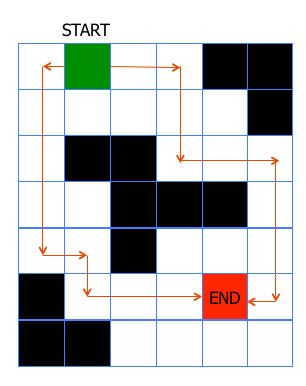
\includegraphics[width=0.5\textwidth]{Figures/grid-path-planning.png}
    \decoRule
    \caption[]{Path Planning Grid}
    \label{fig:PPGrid}
\end{figure}

\subsubsection{Dijkstra Algorithm}
Dijkstra's algorithm is a very generic way to find the path to the goal node which are connected by edges if we consider the configuration space to be a graph. Dijkstra's algorithm was developed by Edsger W. Dijkstra \cite{enwiki:1039157161}. The algorithm
was proposed to solve the path planning by finding the minimum cost path.
\subsubsection{A\textsuperscript{*} Algorithm}
A\textsuperscript{*} algorithm is pretty similar to Dijkstra's algorithm but it has increased performance. Dijkstra's algorithm is a new approach as it starts to explore the global obstacle grid with a starting node and doesn't stop till it reaches the ending node.
It will identify the list of nodes which connect the end node to the starting node to form a path. But there is an issue with Dijkstra, which requires it to explore all the nodes in an equal fashion. This is fine if computation speed and space is not a requirement. 
But exploring all the nodes equally increases the time complexity of the algorithm. If the map is big, using Dijkstra's algorithm can be very computationally expensive. We use A\textsuperscript{*} algorithm to improve the efficiency of search and finding the path.
A\textsuperscript{*} does this by introducing the concept of a \textit{heuristic function} which will help the node exploration towards the goal. The function calculates a correlation of the node to a cost value (a positive value). 
Heuristic functions are calculated by satisfying these basic criteria.

\begin{itemize}
    \item H(goal) = 0
    \item H(x) $<=$ H(y) + cost(x,y), where cost(x,y) is the cost to travel from one node to the other and x,y are the two adjecent nodes. 
\end{itemize}

By keeping the cost of the goal node 0, it helps us increase the cost efficiency because we do not have a direction. Thus, if the cost of travelling from a node to the other can bring us closer to the goal we use it as it increases our exploration time.
Heuristic function cost(x,y) can be calculated by using either Euclidian Distance or Manhattan Distance depending on one's preference. 
\subsubsection{Greedy Best First Search Algorithm}
Greedy Best-First Search (Greedy Best-First Search) Algorithm is a search algorithm. The configuration space is represented as a graph of different nodes. 
The algorithm will explore the whole graph by expanding the nodes which can have promising next nodes according to a rule. Pearl J. \cite{pearlJ} defines GBFS
as an estimation of the most promising next node N by a heuristic evaluation function \textit{f(n)} which, in general, depends on the description of N, the information 
of the goal, the information gathered by the process upto this point, and other knowledge about a problem domain.
Configuration space for GBFS algorithm is accomplished by using Visibility Graph Method. The method states that the path is defined as a line connecting the starting
configuration with the ending goal configuration by employing the non-free configuration space. As we define the non-free configuration paths, possible non-collision paths between the start and goal positions are defined too.
As the information about the robot's workspace increases, the quality of the algorithm increases too. The algorithm will work better when we have much more information about the robot's workspace.

\subsection{Local Planner Algorithms}
Local Planners are dynamic path planning algorithm, which means that the algorithm works online while the robot is moving, unlike global planner algorithms where the next states are already decided and the robot follows the specific path. 
Local Planner Algorithms require constant update and calculation of the values recieved from sensors, wheather it is a LIDAR sensor or a camera vision sensor. The algorithm computes those values returned to predict a short term relapse path towards the goal.
There are several local planner algorithms such as \textit{Dynaamic Window Approach (DWA) local planner}, \textit{Time-Elastic-Band (TEB) local planner} already implemented in the ROS package, which we will discuss about in this section. Local Planner also helps the robot to maintain it's path that was calculated earlier by the global planner algorithm. 
In this subsection, we will discuss about the local path planning algorithms.

\subsubsection{TEB local planner}
Configuration space's representation in TEB local planner is done by using a \textit{Sampling-Based approach}.
The planner uses a novel approach named \textit{Time-Elastic-Band algoritm} for obstacle avoidance purposes.The algorithm is described
in the paper \cite{KELLER20149822}. The motion planning is to move the robot from A(x\textsubscript{o}, y\textsubscript{o}) to B(x\textsubscript{N}, y\textsubscript{N}) without any collision with relation to the global and local reference frames.
The local path planner provides a turn in the angle of rotation in \textit{y} axis and a forward motion to avoid the obstacle. 

TEB (see Figure~\ref{fig:TEBPlanner}) is done by describing a fixed number of points to the final goal, \textit{(x\textsubscript{0}, y\textsubscript{0})}, \textit{(x\textsubscript{1}, y\textsubscript{1})}, \textit{(x\textsubscript{2}, y\textsubscript{2})}\dots \textit{(x\textsubscript{N}, y\textsubscript{N})}
 . The different points are put apart by a time interval. The time interval is the difference in travelling two points. Time Elastic Band is made up from 
two different set of points and the time interval, i.e B = (Q,T) and the time band is computed by minimizing a sum of multiple objectives and cost functions to find the new path to get to the final position. The differences betweent the consecutive points are used to calculate the velocity and acceleration for the robot.

\subsection{DWA local planner}
DWA local planner (see Figure~\ref{fig:DWAPlanner}) stands for using \textit{Dynamic Window Approach} to navigation in a regular updating fashion on the surface. After the global path planner gives a path and a costmap configuration space, the local planner will send the velocity to the robot to avoid any obstacles.
DWA local planner utilises the BaseLocalPlanner interface which is specified in the navigation package. The \textit{dwa local planner} provides a controller to control the mobile motor of the robot. The controller will connect the path planning process to the robot. The robot uses a map to create a planner trajectory to get from the start to goal location.
Grid is created around the robot using the LIDAR sensor. The grid cells are utilized to calculate cost value, and the controller will use utilize the value function to send the values of velocity\textsubscript{x}, velocity\textsubscript{y} and velocity rotation theta to the robot.

Major ideas in Dynamic Window Approach (DWA) are described below : 
\begin{itemize}
    \item Getting values from robot's LIDAR sensor and discretely calculating the robot's control space.
    \item Velocity is calculated from the function to calculate the current state and predicting the next sampled velocity with next state in case of deflection with an obstacle.
    \item The velocity will be applied for a very short period of time.
    \item Different trajectories are generated to avoid the obstacle.
    \item The trajectory with the highest score and providing the lowest cost to move towards the goal is chosen.
    \item The trajectory is chosen, and the associated velocity is sent to the motor by the controller. 
    \item You repeat the algorithm everytime you find an obstacle. 
\end{itemize}

Our choice was to use Dijkstra algorithm for the global planner algorithm and dynamic window approach for the local planner algorithm.
Implementation for A\textsuperscript{*} and GBFS algorithm is also done, and can be implemented based upon preference.

\begin{figure}[th]
    \centering
    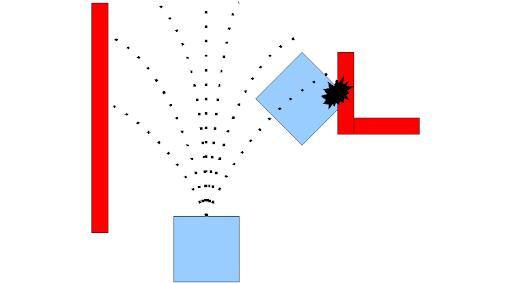
\includegraphics[width=0.9\textwidth]{Figures/dwa_planner.png}
    \decoRule
    \caption[]{DWA Planner}
    \label{fig:DWAPlanner}
\end{figure}

\begin{figure}[th]
    \centering
    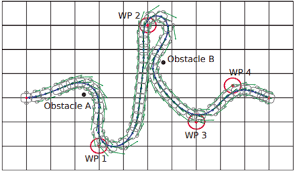
\includegraphics[width=0.9\textwidth]{Figures/TEB.png}
    \decoRule
    \caption[]{TEB Planner}
    \label{fig:TEBPlanner}
\end{figure}


 
%% Chapter Template

\chapter{Implementation} % Main chapter title

\label{Chapter3} % Change X to a consecutive number; for referencing this chapter elsewhere, use \ref{ChapterX}

\section{Introduction}
In the previous chapters, we discussed about the context of the work and the technologies, both software and hardware required to execute the project. In this chapter, we would go through methods and steps 
with which we can utilise those technologies to produce results. In our implementation, we wish to study the behavior of robot with respect to it's neighbourhood obstacles. To achieve studying of goals, we will use the relative position of the robot
with respect to the obsatcles and result in a log file for data mining purposes.

\section{Environment Development}
The simulation environment used in the project is Gazebo11 \cite{1389727}. Gazebo is a simulation environment where we can create a Digital Twin \cite{8901113}. ROS framework utilizes Gazebo as 
the simulation environment for both our robot as well as the obsatcle environment. To simply simulate the robot into Gazebo, we need to define \textit{launch} files, which contain arguments to define the robot and it's specifications.
In a launch file, we define the initial position of the robot, the world file we might use, import the neccesary equipments of the robots and define the sensors of the robot, it's base, and the manufacturer of each.
The equipments are defined by using \textit{xacro} files which are saved in the same directory. We can also call other processes and scripts to run, as well as visualization in the launch file. The \textit{launch} file also helps us define and call \textbf{AMCL} launch file,
which helps us localize the robot in the environment frame. The launch files contain arguments to visualize the processes with RViz (ROS Visualization Tool). The launch file is programmed in XML-like structure.
In the project, we have floor tiles, square boxes and walls surrounding the environment. These entities can be created in CAD and imported as we intend to implement. These entities are stored in \textit{.gazebo} directory 
and therefore can be used to develop other environments with different configurations. The digital twin developed along with the robot is noted and studied from the top at \textit{god's eye view}.
In ROS package, launch folders contain the launch files, which call models from models and world directory. Note that, models are building blocks of world files. World files with different configurations are stored in \textit{worlds} directory in the ROS package.

\begin{figure}[th]
    \centering
    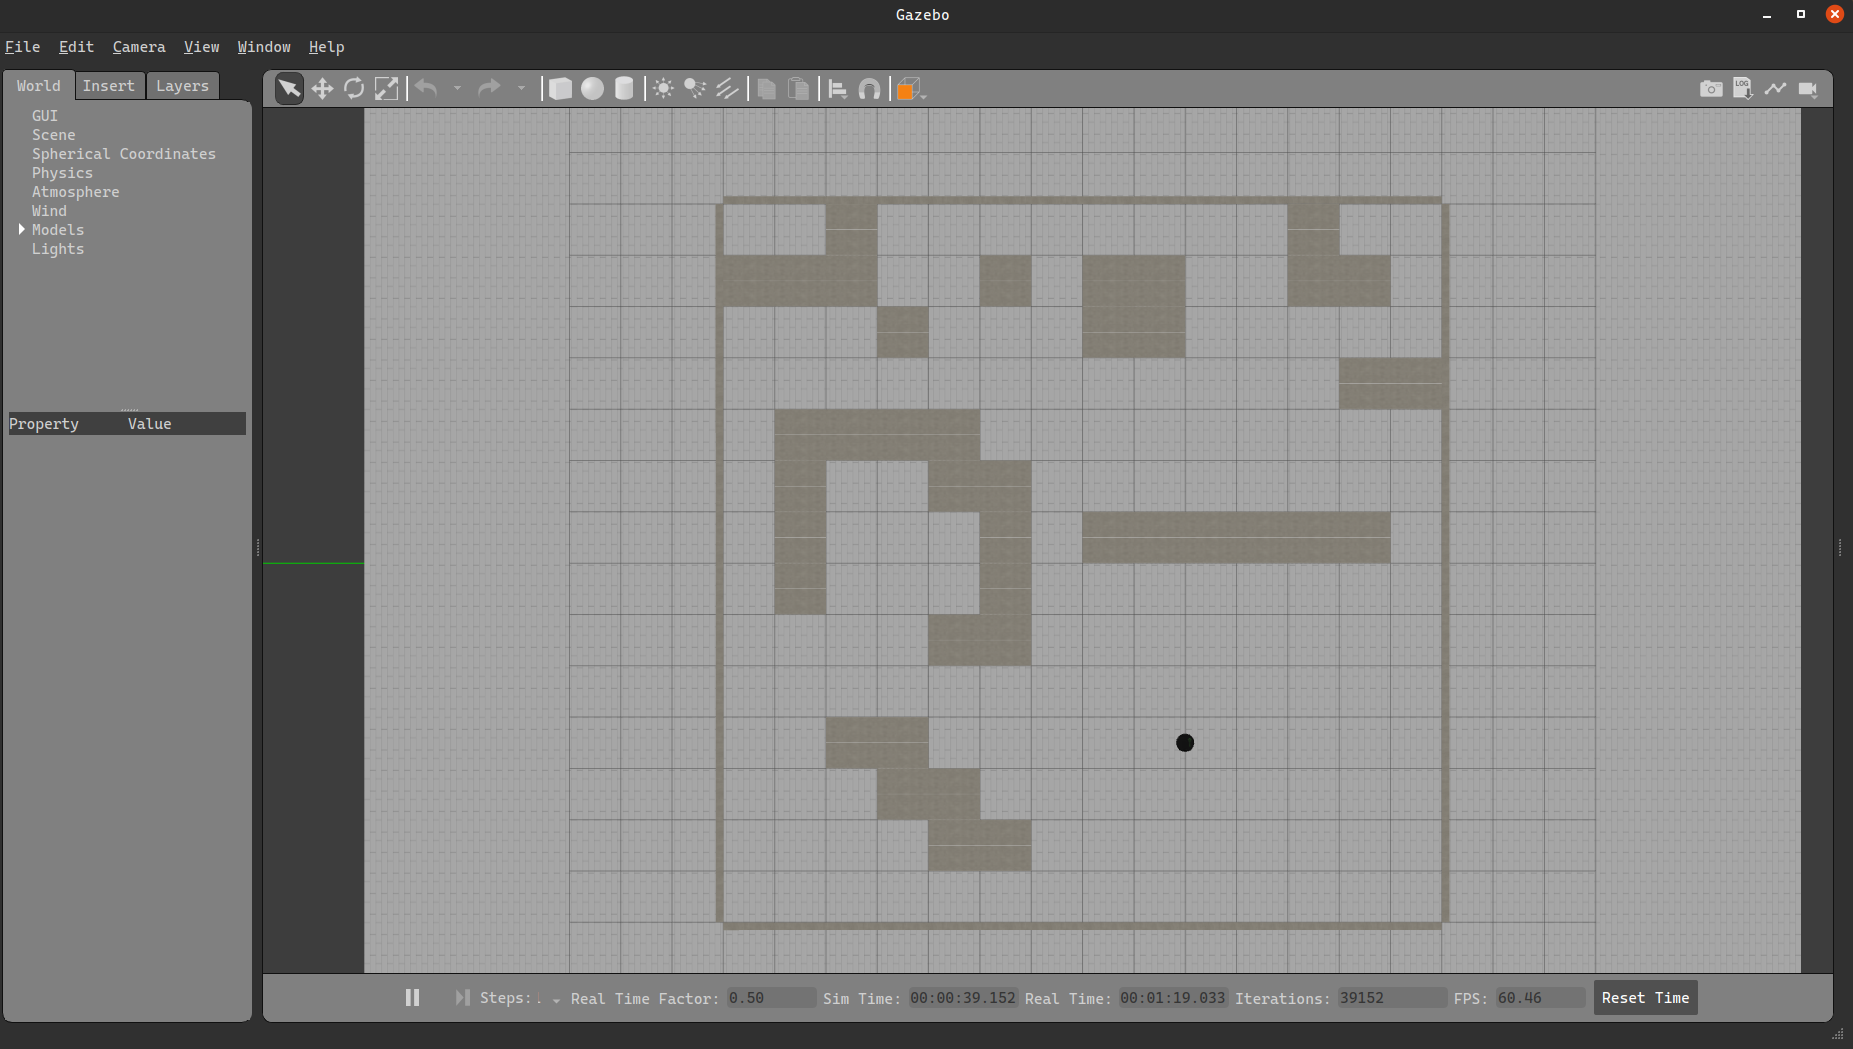
\includegraphics[width=\textwidth]{Figures/base_god_eye_world.png}
    \decoRule
    \caption[]{God's eye view of 14x14 grid}
    \label{fig:14x14grid}
\end{figure}

\begin{figure}[th]
    \centering
    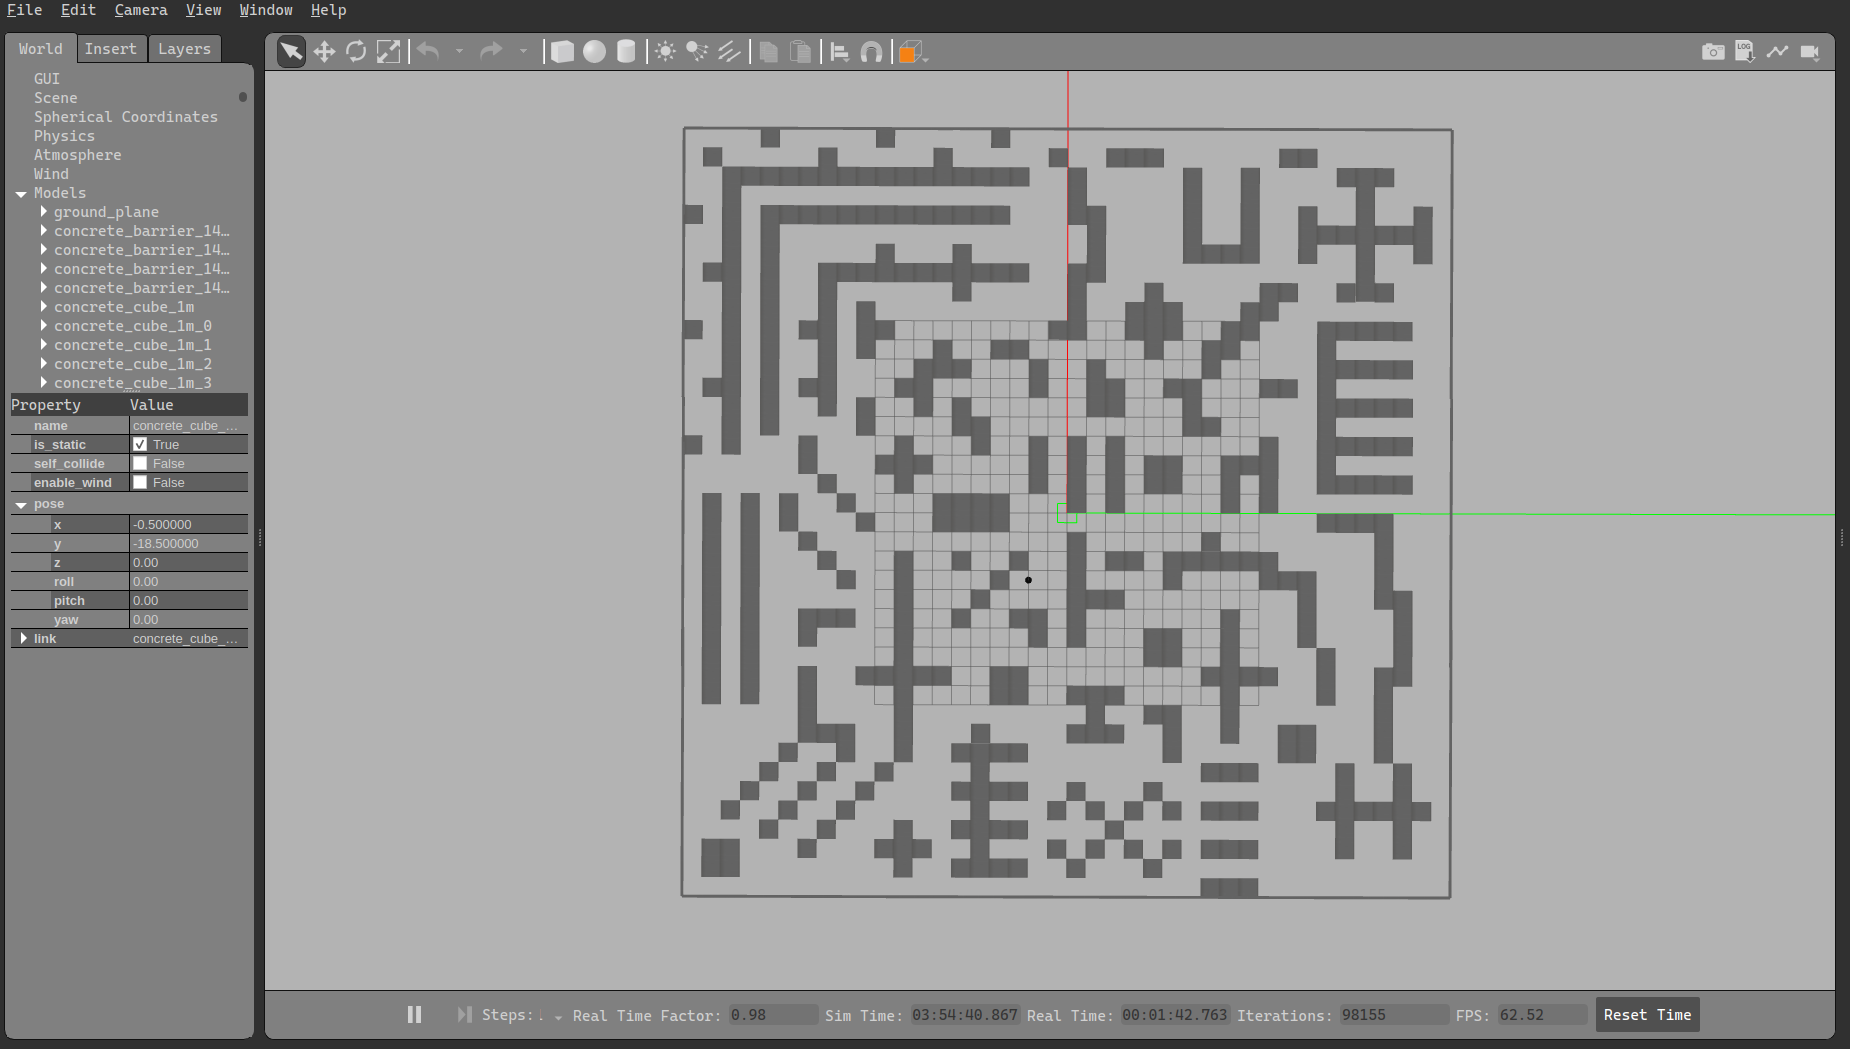
\includegraphics[width=\textwidth]{Figures/30_30_god_eye_world.png}
    \decoRule
    \caption[]{God's eye view of 30x30 grid}
    \label{fig:30x30grid}
\end{figure}

\section{SLAM}
SLAM (Simultaneous Localization and Mapping) is done by simulating the turtlebot in a particular environment. 
As the robot does not know anything about the environment, a \textit{teleoperation} command, i.e using the keyboard
to move the robot around the environment. As the robot has a 360\textsuperscript{o} LIDAR sensor, concurrent mapping 
and localization is done. The map is generated and saved for further global path planning and navigation.The user, controlling the 
robot stop the teleoperation will stop moving around the robot when the mapping is done completely.
In SLAM methods in ROS, we can use different methods to execute SLAM such as "gmappping" (\url{wiki.ros.org/gmapping}) which uses a two
dimensional occupancy grid map describing the configuration space. Another such method is "cartographer" (\url{wiki.ros.org/cartographer})
utilizing an algorithm employing loop closure method. In our work, we implemented the \textit{gmapping} package to implement SLAM.

\begin{itemize}
    \item Simulate the robot in environment with \textit{launch} files.
    \item Using turtlebot package to initiate SLAM.
    \item Starting the teleoperation node in another terminal.
    \item Moving the robot around the environment to record the map.
    \item Saving the map.
\end{itemize}

\begin{figure}[th]
    \centering
    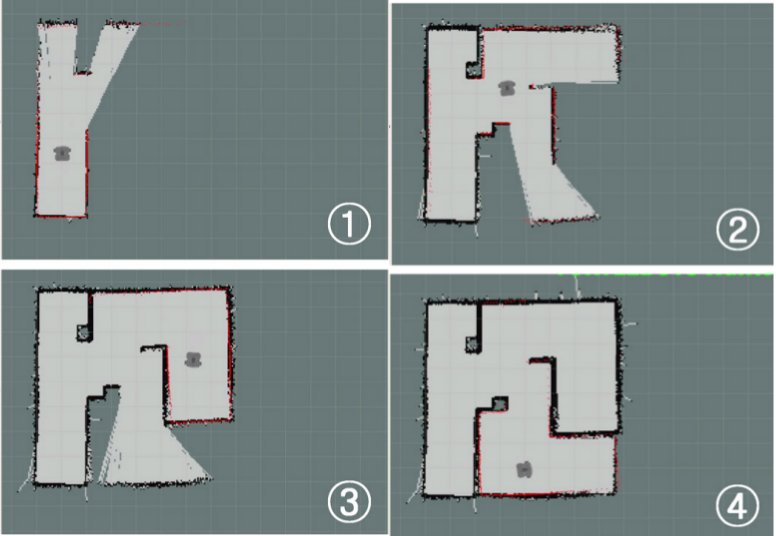
\includegraphics[width=\textwidth]{Figures/SLAM.png}
    \decoRule
    \caption[]{Step-by-Step SLAM}
    \label{fig:Step-by-StepSLAM}
\end{figure}

\section{Navigation}
Navigation in ROS based environment is done through the navigation stack. Navigation stack is an open-source framework in ROS which accompanies everthing 
required for a robot to move from a point to the other. The navigation stack is completely configurable, and developer can add 
their code into the stack when we wish to. Navigation stack is available on Github, for anyone to use and utilise. 
ROS Navigation stack is on a conceptual level. The information is taken from odometry, and goal pose of the robot and sensors. 
Navigation stack deals with publishing velocity to the robot controller, the values will be published
according to the need to reach the goal pose. There are many prerequisites in Navigation Stack, 
\begin{itemize}
    \item The robot should be running ROS.
    \item coordinate frame of the robot, i.e \textit{tf transforms} should be known.
    \item global plan coordinate frame of the robot should be known.
    \item correct \textit{message} files to exchange information in between processes.
\end{itemize}
To fully setup the essential navigation stack, it's configuration can be done through \url{http://wiki.ros.org/navigation}
In our implementation, we are using the local path planner but we are not employing the LIDAR sensor to avoid obstacle dynamically.
The robot in our implementation, does not intend to path plan in a dynamic fashion. Instead, we wish to read the behaviour of the robot in relation with it's global path plan.
In the data flow in Navigation Stack, odometry and LIDAR are the chosen combination. Odometry is the most important information in the control.
As we wish to \textit{see and record} the behavior of the robot from a god's eye view, we will only use Odometry information to
see the \textit{x and y} values of the robot in relation to the coordinate frame. The goal pose is chosen from using the ROS Visualization tool.
Navigation stack will be turned on to work, when a goal pose is chosen. The navigation then publishes the trajectory poses and velocity from the 
robot's controller. The transform tree, is utilized to specify the motion constraints of the robot like it's height and width of the mobile base.
There are various such parameters attached in the \textit{config} folder describing different patterns in numerous \textit{.yaml} files.

\subsection{Customized Global Planner Algorithm}
In our implementation, the robot's possible movements are only in 4 directions. We don not wish the optimization of the path, instead we wish to focus
on defining the movement in those directions. Thus, after defining the \textit{global costmap} and it's grids. The algorithms should only iterate and explore
over the \textit{top, left, right and down} nodes only at each and every step.
In the figure 3.4, the node \textbf{R} is an obstacle, which is describe as a value greater than 1 in global costmap configuration.
Thus, the robot's global planner can not explore that node and further nodes that can exist and explored from using \textbf{R} as a referemce point.
As the nodes \textbf{L,P and V} are free, in the next step the robot's global planner will proceed to explore the other nodes built upon those.
\begin{figure}[th]
    \centering
    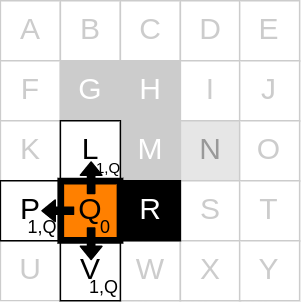
\includegraphics[width=0.4\textwidth]{Figures/grid_map_expansion_02.png}
    \decoRule
    \caption[]{Exploration Strategy of Nodes}
    \label{fig:NodeExploration4Node}
\end{figure}
Let's consider that \textbf{L} was node chosen in order to move to the goal pose. We will proceed to explore the nodes adjecent to the \textbf{L} node.
In figure 3.5, the node \text{L} has 4 neighbours, namely \textbf{K,G,M,Q}. As \textbf{G and M} are obstacles with \textbf{Q} being the previous explored node.
We have no other option to chose node K as our next node.

\subsubsection{Strategies of Planning}
As we discussed that, there are three algorithms implemented in our project which are namely, \textit{Dijkstra's Algorithm, A\textsuperscript{*} Algorithm and GBFS algorithm}.
These three algorithms will follow a similar node exploration strategy but the incentives to explore a new node will differ from algorithm to algorithm, resulting in different strategies to reach the goal pose node.

\begin{figure}[th]
    \centering
    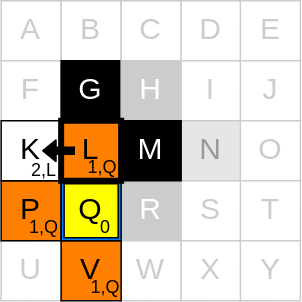
\includegraphics[width=0.4\textwidth]{Figures/grid_map_expansion_03.png}
    \decoRule
    \caption[]{Next stage of exploration.}
    \label{fig:NextNodeExploration4Node}
\end{figure}







%% Chapter Template

\chapter{Solution to Log Generation} % Main chapter title

\label{Chapter4} % Change X to a consecutive number; for referencing this chapter elsewhere, use \ref{ChapterX}

\section{Introduction}
In the previous chapters, we have discussed the method to implement the solution to generate a path. Path Generation and Implementation of a method to store the behaviour of the robot with respect to it's neighbours is another issue.
In this chapter, we will cover the method implemented for generation of the log file with respect to the nearby obstacles. 

\section{Constraints}
As we are implementing the solution by following the hypothesis that we wish to see and generate the log in the Digital Twin from the perspective of the God's eye.
We can not use any information that has been published by the robot. Thus, we can not use \textit{scan} topic and sensors to infer data and proceed with data mining.
Therefore, we are only limited to \textit{'use what we can see'}. Odometry describe the position of the robot in the context of the environment. From the god's eye perspective,
we can only see the positional information or \textit{position} of the robot. Therefore, to solve the log generation problem we will only use the \textbf{x} and \textbf{y} positions of the robot.

\section{Using Odometry}
Odometry is a \textit{topic} in ROS which describes the postion of the robot in the coorrdinate system. Odometry message type contains :
\begin{itemize}
    \item \textbf{std\_msgs/Header \textit{header}}, providing a header to the information.
    \item \textbf{string child\_frame\_id}, providing the ID to the frame generated from positional transforms of the robot model.
    \item \textbf{PoseWithCovariance}, describing the linear positional information about the robot i.e the x,y,z position of the robot in the coorrdinate frame.
    \item \textbf{TwistWithCovariance}, describing the angular positional information about the robot i.e the x,y,z angular rotation in the coorrdinate frame.
\end{itemize}

Odometry is the best choice for generation of log file in our implementation. This is because, in our hypothesis, the values should be recorded from the god's eye view (see Figure~\ref{fig:DigitalTwinGodEye}).
Implementation can be done from the robot's LIDAR sensor, although we will get the values from the robot. This implementation will deviate us from our hypothesis. In implementation with the LIDAR sensor, we found out that
the values were not regular. This could be due to incompetency of the LIDAR sensor. We needed to find a different definitive method, using values from odometry. 
In the Figure~\ref{fig:LIDARSensorGrid}, the light grey grid is generated with LIDAR sensor. The process is continous, and not positional. This results in varying discrepency in the data generated. We recorded loss in data, making this approach unusable and further solidifying 
the use of odometry.

\begin{figure}[th]
    \centering
    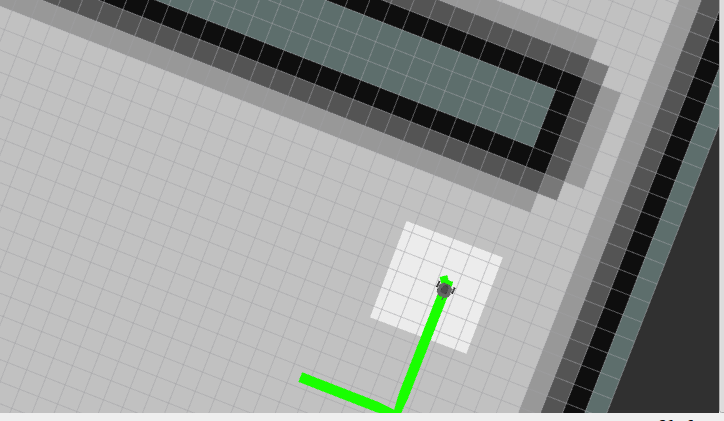
\includegraphics[width=\textwidth]{Figures/local_costmap-grid.png}
    \decoRule
    \caption[]{Grid Generated by Robot}
    \label{fig:LIDARSensorGrid}
\end{figure}

\section{Solution}

\subsection{Obstacle Space}
While generation of the environment in Gazebo, every obstacle is given a position in it. The position of the obstacle is also described by 
using \textbf{x} and \textbf{y} positions of the obstacle. Thus, if we have 44 boxes, we should have 44 different pairs of \textbf{x} and \textbf{y} positions for the obstacle space.
\begin{figure}[th]
    \centering
    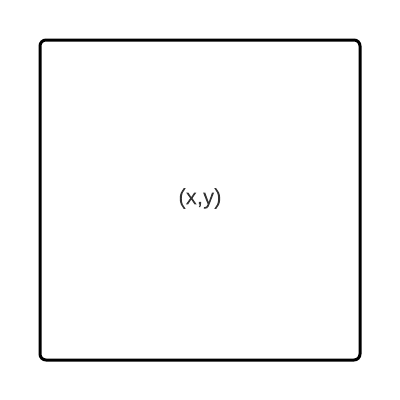
\includegraphics[width=0.3\textwidth]{Figures/simple-obstacle-x-y.png}
    \decoRule
    \caption[]{Obstacle positioning}
    \label{fig:ObstaclePositioning}
\end{figure}

We implemented the log generation algorithm using just 44 different boxes and 44 pairs of \textbf{x} and \textbf{y} positions. We rounded the \textbf{x} and \textbf{y} position to the nearest \textit{point 5}
To generate a 3 by 3 grid, we calculated if the \textbf{x} and \textbf{y} poisitions and adding 0.5 to the values collides with the center of the robot. The method was basic, produced results but was not accurate 
and thus was not suitable for our implementation. We had to increase the number of contact points and change the algorithm, see \ref{finalsol}.

\subsubsection{Correlation of obstacle with robot}
In our digital twin, we wish to use the Odometry positions of the robot as well as the obstacles around the robot. To find if there is an obstacle near the robot, we will have to find a way to correlate the both positions.
A simple algorithm to do so could be,
\begin{itemize}
    \item Finding the x, y position of the robot.
    \item Using the distance of the center of the obstacle with it's borders.
    \item Adding the particular value to the obstacle's position
    \item If it is equal, obstacle is there else not.
    \item Recording this behaviour.
\end{itemize}

The algorithm can be used to produce the obstacle space in a grid around the robot. The algorithm is simple in it's definition but lacks in many use cases.
For example, if the robot just passes around the corner of the obstacle, the algorithm will not be able to show if the position is close to an obstacle or not.
Thus, it needs improvement. 

The improvement should be noted in correlation to the constraints so solve the problem, i.e by only using the position of the robot as well as the obstacle.

\section{Final Solution}\label{finalsol}
In our implementation, the length of the obstacle is 1 unit. Since the obstacle is a square, the length as well as the breadth are 1 unit each.
There is only one position of the obstalcle i.e at the middle (see Figure~\ref{fig:ObstaclePositioning}). We need to improve on the position, and create more pairs of positions where the obstacle is.
We approached this problem by dividing a square into 8 parts with different positional points. The obstacle's distance from the center to an edge is \textbf{0.5 units}.
In order to improve and give more information about the obstacle space to the robot, we had to divide the obstacle into 8 lines with 5 points on each, signifying the coordinates of the obstacle space.
Each of these points are situated at \textbf{0.1 unit} distance from one another. 

\begin{figure}[th]
    \centering
    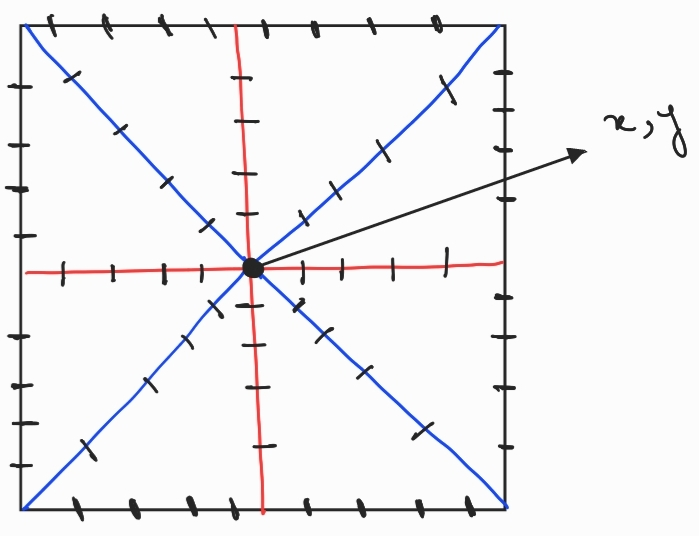
\includegraphics[width=0.4\textwidth]{Figures/improved-obstacle-space.jpg}
    \decoRule
    \caption[]{Divided Obstacle Space}
    \label{fig:ObstacleSpaceDivided}
\end{figure}

As seen in Figure~\ref{fig:ObstacleSpaceDivided}, there are multiple points described in an obstacle space as compared to just one in the previous approach.
Eventhough, we are not using any sensors to get the information, we can name a \textit{perception} range defining the points the robot will check in order to find a point that is present in the obstacle space.
There are 44 obstacles with 72 points each, which means that the obstacle space data structure (python list in our implementation) contains, 3168 pairs of \textbf{x} and \textbf{y} positions.
As the robot will move across the configuration space, the x and y coordinates of the robot will be used to calculate a nearby obsatcle point, if it exists based upon the \textit{perception range} defined in the algorithm.
The obstacle space is saved in a list, and the algorithm will find a point in the perception range of the robot and if it is present in the obstacle space, it will denote it as an obstacle.
Another list will is created, which saves the position values in different grid sizes based upon the perception range of the robot. For example, in a \textit{3 by 3 grid}, the different positions are written to the list, and further to a semi-structured csv file. The log file is then to be used for data mining and reinforcement learning applications.
The log will contain :  

\begin{itemize}
    \item ROS timestamp in seconds.
    \item x and y coordinate of the robot.
    \item the obstacle grid (\textit{any size}) calculated by the algorithm.
    \item x and y coordinates of the goal.
    \item relative x and y coordinates to the goal
    \item manhattan distance of the robot to the goal.
    \item euclidian distance of the robot to the goal.
    \item angular orientation in z axis i.e the rotation of the robot.
\end{itemize}

\section{Conclusion and Perspective}
In this work, we had to develop a method to record the behavior of the robot in an environment with obstacles. We developed a method to navigate a robot from a position to goal position. We implemented different methods to generate the log file, and decide upon using positional values of robot as well as environment's entities to develop the obstacle space around the robot.
The advantage of the method is we can expand it to any size of the grid. To implement this, I had to learn about autonomous navigation of the robot in an environment with ROS. I learnt about digital twins and methods to implement digital twins for behavioural learning. 
The goal of the work was to study the behavior of the robot around different obstacles. Development of navigation methods and an algorithm to infer the data to produce logs was required in completion.
By producing the method for behavioral learning, the work can be expanded for multiple robots as digital twins to learn their behaviour in relation to one another. The generated log file can be used for machine learning, training or testing the developed strategy with digital twins. 
%\include{Chapters/Chapter5} 

%----------------------------------------------------------------------------------------
%	THESIS CONTENT - APPENDICES
%----------------------------------------------------------------------------------------

\appendix % Cue to tell LaTeX that the following "chapters" are Appendices

% Include the appendices of the thesis as separate files from the Appendices folder
% Uncomment the lines as you write the Appendices

% Appendix A

\chapter{Parameters for Navigation} % Main appendix title

\label{Appendix1} % For referencing this appendix elsewhere, use \ref{AppendixA}

\section{Robot's Parameters}
\begin{table*}[ht]
    \caption{Parameters for Costmap}
    \centering
    \begin{tabular}{p{0.25\linewidth}p{0.25\linewidth}}
    \hline
    Parameter & Value \\
    \hline
    max\_obstacle\_height & 0.60\\
    robot\_radius & 0.17\\
    \\
    obstacle\_layer & : \\
    enabled & true \\
    max\_obstacle\_height & 0.6 \\
    origin\_z & 0.0 \\
    z\_resolution & 0.2 \\
    z\_vowels & 10 \\
    unknown\_threshold & 15 \\
    mark\_threshold & 0 \\
    combination\_method & : 1\\
    track\_unknown\_space & true \\
    obstacle\_range : 5.5\\
    raytrace\_range : 6.0 \\
    origin\_z & 0.0 \\
    publish\_voxel\_map & false \\
    observation\_sources & scan \\
    \\
    inflation\_layer & : \\
    enabled & true \\
    cost\_scaling\_factor : 5.0 \\
    inflation\_radius : 0.4 \\
    static\_layer & : \\
    enabled & true \\
    \hline
    \end{tabular}
\end{table*}

\begin{table*}[ht]
    \caption{Global Costmap Parameters}
    \centering
    \begin{tabular}{p{0.25\linewidth}p{0.25\linewidth}}
        \hline
        Parameter & Value \\
        \hline
        global\_frame & map \\
        robot\_base\_frame & base\_footprint \\
        update\_frequency & 0.2 \\
        publish\_frequency & 0.2 \\
        transform\_tolerance & 0.5 \\
    \end{tabular}
\end{table*}

\begin{table*}[ht]
    \caption{Global Planner Parameters}
    \centering
    \begin{tabular}{p{0.25\linewidth}p{0.25\linewidth}}
        \hline
        Parameter & Value \\
        \hline
        old\_navfn\_behavior & false \\
        use\_quadratic & true \\
        use\_dijkstra & true \\
        use\_grid\_path & false \\
        allow\_unknown & true \\
        planner\_window\_x & 0.0 \\
        planner\_window\_y & 0.0 \\
        default\_tolerance & 0.0 \\
        publish\_scale & 100 \\
        lethal\_cost & 253 \\
        neutral\_cost & 50 \\
        cost\_factor & 3.0 \\
        publish\_potential & true \\
     \end{tabular}   
\end{table*}


%\include{Appendices/AppendixB}
%\include{Appendices/AppendixC}

%----------------------------------------------------------------------------------------
%	BIBLIOGRAPHY
%----------------------------------------------------------------------------------------

\printbibliography[heading=bibintoc]

%----------------------------------------------------------------------------------------

\end{document}  
